\begin{exercise}{2016/17 7}
    \emph{Βέλτιστος έλεγχος και Χαμιλτονιανά συστήματα}: Συνοπτικά, εάν έχουμε
    αφινικό σύστημα ελέγχου
    \[
        \dot{x} = f(x) + g(x)u, \quad x \in \mathbb{R}^n, u \in \mathbb{R}^m,
    \]
    με \( g(x) n \times m \) πίνακα σταθερού βαθμού \( m \) και θεωρήσουμε
    συναρτησιακό κόστους με \tl{Lagrangian} \( L(x, u) \) (θετικά ορισμένη στο
    \( u \)), σχηματίζουμε την Χαμιλτονιανή
    \[
        H(x, u, p) = \left( f(x) + g(x)u \right)\cdot p - L(x, u),
    \]
    όπου \( p \in \mathbb{R}^n \) δυϊκές μεταβλητές
    (\enquote*{πολλαπλασιαστές \tl{Lagrange}}).

    Η αρχή μεγίστου (ή ελαχίστου) του \tl{Pontryagin} οδηγεί στη βέλτιστη
    Χαμιλτονιανή
    \[
    H^*(x, p) = \underset{u}\sup \, H(x, u, p).
    \]
    Συνήθως, αυτό μας δίνει τον βέλτιστο έλεγχο ως συνάρτηση των \( x \) και
    \( p, u^*(x, p) \). Εάν κάποιες επιπλέον συνθήκες ισχύουν, τότε οι βέλτιστες
    λύσεις \( (x(t), p(t)) \) είναι οι τροχιές του Χαμιλτονιανού συστήματος για
    τη συνάρτηση \( H^* \).
    \begin{enumerate}[label= (\alph*)]
        \item Βρείτε τον βέλτιστο έλεγχο \( u^* \) και την \( H^* \) για
            γραμμικά συστήματα,
            \[
                \dot{x} = Ax + Bu, \quad \rank{B} = m
            \]
            και για \tl{Lagrangian}
            \[
                L(x, u) = \frac{1}{2}x^{T}Rx + \frac{1}{2}u^{T}Qu, \quad R \geq
                0, Q >0
            \]
            και δώστε τις Χαμιλτονιανές του εξισώσεις (που πρέπει να είναι
            γραμμικές!).
        \item Μελετήστε το σύστημα σε μία διάσταση \( \dot{x} = ax + bu (b \neq
            0) \) και βρείτε τις λύσεις \( (x, p) \) για την ασταθή περίπτωση \(
            a > 0 \).
    \end{enumerate}
\end{exercise}
\begin{solution}{2016/17 7}
    (α). Για να συμβαδίσω με τους συμβολισμούς που έχω συνηθίσει μέχρι τώρα θα ορίσω
    τη \tl{Lagrangian} ως
    \[
        L(x, u) = \frac{1}{2}x^{T}Qx + \frac{1}{2}u^{T}Ru, \quad Q \geq
        0, R > 0,
    \]
    δηλαδή θα αλλάξω το \( Q \) με το \( R \) και θα ακολουθήσουμε τη διαδικασία
    για την αρχή του ελαχίστου.

    Θεωρούμε την επαυξημένη \tl{Lagrangian}
    \begin{align}\label{eq:ex7_aug_lag}
        L_a(x, u) &= L(x, u) + p^T\left( Ax + Bu - \dot{x} \right) \nonumber \\
        &= \frac{1}{2}x^{T}Qx + \frac{1}{2}u^{T}Ru + p^T\left( Ax + Bu - \dot{x}
        \right).
    \end{align}
    Από το λογισμό των μεταβολών είναι γνωστό ότι, οι αναγκαίες συνθήκες για την
    ύπαρξη ακρότατου είναι να ικανοποιούνται οι εξισώσεις \tl{Euler-Lagrange}.
    Έτσι για τη σχέση~\eqref{eq:ex7_aug_lag} πρέπει να ισχύει
    \begin{align}
        0 &= \frac{\partial L_a}{\partial p}(x^*, u^*, p^*) -
        \frac{d}{dt}\left(
        \frac{\partial L_a}{\partial \dot{p}}(x^*, u^*, p^*)\right)
        \label{eq:ex7_eul_lag_p}\\
        0 &= \frac{\partial L_a}{\partial x}(x^*, u^*, p^*) -
        \frac{d}{dt}\left(
        \frac{\partial L_a}{\partial \dot{x}}(x^*, u^*, p^*)\right)
        \label{eq:ex7_eul_lag_x}\\
        0 &= \frac{\partial L_a}{\partial u}(x^*, u^*, p^*) -
        \frac{d}{dt}\left(
        \frac{\partial L_a}{\partial \dot{u}}(x^*, u^*, p^*)\right).
        \label{eq:ex7_eul_lag_u}
    \end{align}
    Ορίζουμε την Χαμιλτονιανή ως
    \begin{align}\label{eq:ex7_hamilton}
        H(x, u, p) &= L(x, u) + p^T\left(Ax + Bu\right) \nonumber \\
        &= \frac{1}{2}x^{T}Qx + \frac{1}{2}u^{T}Ru + p^T\left( Ax + Bu \right).
    \end{align}
    Με αντικατάσταση της \( L(x, u) \) από τη σχέση~\eqref{eq:ex7_aug_lag}
    \[
        L(x ,u) = L_a(x, u, p) - p^T\left(Ax + Bu - \dot{x} \right),
    \]
    θα έχουμε
    \[
        H(x, u, p) = L_a(x, u, p) - p^T\left( Ax + Bu - \dot{x} \right)
        + p^T\left( Ax + Bu \right),
    \]
    και τελικά προκύπτει
    \[
        L_a(x, u, p) = H(x, u, p) - p^{T}\dot{x}.
    \]
    Έτσι από τη σχέση~\eqref{eq:ex7_eul_lag_p} προκύπτει
    \begin{align*}
        0 &= \frac{\partial H(x^*, u^*, p^*) - p^{T}\dot{x}}{\partial p} -
        \frac{d}{dt}\left(
        \frac{\partial H(x^*, u^*, p^*) - p^{T}\dot{x}}{\partial \dot{p}}\right)
        \\
        0 &= \frac{\partial H}{\partial p} (x^*, u^*, p^*) - \dot{x},
    \end{align*}
    που οδηγεί στη σχέση
    \begin{equation}\label{eq:ex7_Hx_star}
        \dot{x}^* = \frac{\partial H}{\partial p} (x^*, u^*, p^*).
    \end{equation}
    Αντίστοιχα από τη σχέση~\eqref{eq:ex7_eul_lag_x} προκύπτει
    \begin{align*}
        0 &= \frac{\partial H(x^*, u^*, p^*) - p^{T}\dot{x}}{\partial x} -
        \frac{d}{dt}\left(
        \frac{\partial H(x^*, u^*, p^*) - p^{T}\dot{x}}{\partial \dot{x}}\right)
        \\
        0 &= \frac{\partial H}{\partial x} (x^*, u^*, p^*) - \frac{d}{dt}(-p),
    \end{align*}
    που οδηγεί στη σχέση
    \begin{equation}\label{eq:ex7_Hp_star}
        \dot{p}^* = -\frac{\partial H}{\partial x} (x^*, u^*, p^*).
    \end{equation}
    Τέλος, από τη σχέση~\eqref{eq:ex7_eul_lag_x} προκύπτει
    \[
        0 = \frac{\partial H(x^*, u^*, p^*) - p^{T}\dot{x}}{\partial u} -
        \frac{d}{dt}\left(
        \frac{\partial H(x^*, u^*, p^*) - p^{T}\dot{x}}{\partial \dot{u}}\right)
    \]
    που οδηγεί στη σχέση
    \begin{equation}\label{eq:ex7_Hu_star}
        0 = \frac{\partial H}{\partial u} (x^*, u^*, p^*).
    \end{equation}

    Από τη σχέση~\eqref{eq:ex7_Hu_star} προκύπτει
    \begin{align*}
        0 &= \frac{\partial H}{\partial u} (x^*, u^*, p^*) \\
        &= Ru^* + B^{T}p^*,
    \end{align*}
    που οδηγεί στον βέλτιστο έλεγχο
    \begin{equation}\label{eq:ex7_u_star}
        u^* = -R^{-1}B^{T}p^*.
    \end{equation}
    Από τη σχέση~\eqref{eq:ex7_Hp_star} προκύπτει
    \begin{align}\label{eq:ex7_p_star}
        \dot{p}^* &= -\frac{\partial H}{\partial x} (x^*, u^*, p^*) \nonumber \\
        \dot{p}^* &= -\left(Qx^* + A^{T}p^*\right) \nonumber \\
        \dot{p}^* &= -Qx^* - A^{T}p^*.
    \end{align}
    Από τη σχέση~\eqref{eq:ex7_Hx_star} προκύπτει
    \begin{align}\label{eq:ex7_x_star}
        \dot{x}^* &= \frac{\partial H}{\partial p} (x^*, u^*, p^*) \nonumber \\
        \dot{x}^* &= Ax^* + Bu^*,
    \end{align}
    που οδηγεί στους περιορισμούς του προβλήματος. Με αντικατάσταση
    της~\eqref{eq:ex7_u_star} στην~\eqref{eq:ex7_x_star} προκύπτει
    \[
        \dot{x}^* = Ax^* - BR^{-1}B^{T}p^*.
    \]
    Από την παραπάνω σε συνδυασμό με τη σχέση~\eqref{eq:ex7_p_star} προκύπτει
    ένα σύστημα γραμμικών κανονικών διαφορικών πρώτης τάξης ως προς
    \( x^* \) και \( p^* \)
    \begin{equation}\label{eq:ex7_xp_sys}
        \begin{pmatrix}
            \dot{x}^* \\
            \dot{p}^*
        \end{pmatrix} =
        \begin{pmatrix}
            A & -BR^{-1}B^{T} \\
            -Q & -A^{T}
        \end{pmatrix}
        \begin{pmatrix}
            x^* \\
            p^*
        \end{pmatrix}.
    \end{equation}
    Επίλυση του παραπάνω συστήματος~\eqref{eq:ex7_xp_sys} καθώς και από τη
    σχέση~\eqref{eq:ex7_u_star} βρίσκουμε τις βέλτιστες καταστάσεις, τους
    βέλτιστους πολλαπλασιαστές \tl{Lagrange} καθώς και το βέλτιστο έλεγχο,
    αντίστοιχα. Τέλος, με αντικατάσταση αυτών στη σχέση της
    Χαμιλτονιανής~\eqref{eq:ex7_hamilton}, προκύπτει η βέλτιστη τιμή της \( H^*
    \).

    (β). Θα εφαρμόσουμε τα παραπάνω στο σύστημα \( \dot{x} = ax + bu \) με \( a >
    0 \) και \( b \neq 0 \). Έτσι η Χαμιλτονιανή θα είναι
    \[
        H(x, u, p) = \frac{1}{2}qx^2 + \frac{1}{2}ru^2 + p(ax + bu).
    \]
    Ο βέλτιστος έλεγχος θα είναι
    \[
        u^* = -\frac{b}{r}p^*.
    \]
    Για να βρω το βέλτιστο έλεγχο θα πρέπει να λύσω το σύστημα
    \begin{equation*}
        \begin{pmatrix}
            \dot{x}^* \\
            \dot{p}^*
        \end{pmatrix} =
        \begin{pmatrix}
            a & -\frac{b^2}{r} \\
            -q & -a
        \end{pmatrix}
        \begin{pmatrix}
            x^* \\
            p^*
        \end{pmatrix} = A
        \begin{pmatrix}
            x^* \\
            p^*
        \end{pmatrix}.
    \end{equation*}
    Ένας τρόπος για να βρούμε τις οριακές συνθήκες είναι ο εξής. Αν επιθυμούμε
    η κατάσταση \( x \) να πάει στο μηδέν στο τελικό χρόνο, τότε
    για γνωστή αρχική συνθήκη και καθορισμένο τελικό χρόνο, μπορούμε να
    υπολογίσουμε την αρχική συνθήκη για τον πολλαπλασιαστή \tl{Lagrange}. Έτσι
    λύση της παραπάνω για τελικό χρόνο \( t_f \) είναι
    \begin{equation*}
        \begin{pmatrix}
            x^*(t_f) \\
            p^*(t_f)
        \end{pmatrix} =
        e^{At_f}
        \begin{pmatrix}
            x(t_0) \\
            p(t_0)
        \end{pmatrix} =
        \begin{pmatrix}
            h & j \\
            k & l
        \end{pmatrix}
        \begin{pmatrix}
            x(t_0) \\
            p(t_0)
        \end{pmatrix}.
    \end{equation*}
    Άρα η πρώτη σχέση από το παραπάνω σύστημα δίνει
    \[
        x^*(t_f) = hx_0 + j p_0,
    \]
    που σημαίνει
    \[
        p_0 = \frac{x^*(t_f) - hx_0}{j}.
    \]

    Το σύστημα διότι είναι σε μικρές διαστάσεις έχει αναλυτική λύση που θα
    γράψουμε παρακάτω. Γενικά, αναλυτικές λύσεις δεν μπορούμε να βρούμε, παρά
    μόνο όταν είναι τόσο απλά συστήματα.
    \begin{align*}
        x^*(t) &= \frac{
            \sqrt{r}wc_2\cosh{vt} + (b^2c_1 + arc_2)\sinh{vt}
        }{\sqrt{r}w} \\
        p^*(t) &= \frac{
            wc_1\cosh{vt} - \sqrt{r}(ac_1 + qc_2)\sinh{vt}
        }{w},
    \end{align*}
    όπου \( c_1, c_2 \) είναι οι σταθερές ολοκλήρωσης και υπολογίζονται από τις
    οριακές συνθήκες και \(w, v \) είναι
    \[
        w = \sqrt{b^2q + a^2r}, \quad v = \sqrt{\frac{b^2q + a^2r}{r}}.
    \]

    Στο σχήμα~\ref{fig:ex7_case1} βλέπουμε μία λύση του συστήματος. Οι
    παράμετροι έχουν επιλεγεί ως \( a = 2, b = 1, q = 1, r = 0.25 \), ακόμη η
    αρχική συνθήκη για το \( x_0 = 5 \) και επιθυμούμε η κατάσταση να φτάσει στο
    μηδέν.
    \begin{figure}[h]
        \centering
        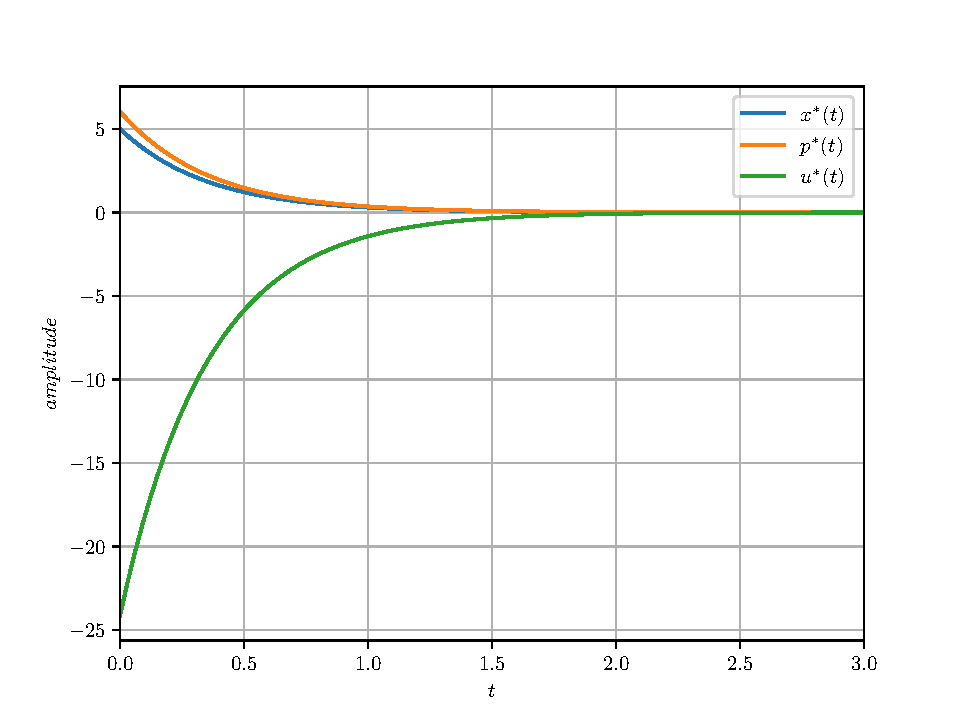
\includegraphics[width=0.9\textwidth]{figures/ex7_case1.pdf}
        \caption{\gr{Βέλτιστες τροχιές,
        \( a = 2, b = 1, q = 1, r = 0.25 \)}}
        \label{fig:ex7_case1}
    \end{figure}
\end{solution}
